\documentclass[border=10pt]{standalone}
\usepackage[svgnames]{xcolor}
\usepackage{amsmath}
\usepackage{pgfplots}
\pgfplotsset{compat=newest}
\usepackage[sfdefault]{FiraSans}
\usepackage{FiraMono}
\renewcommand*\familydefault{\sfdefault}
\begin{document}
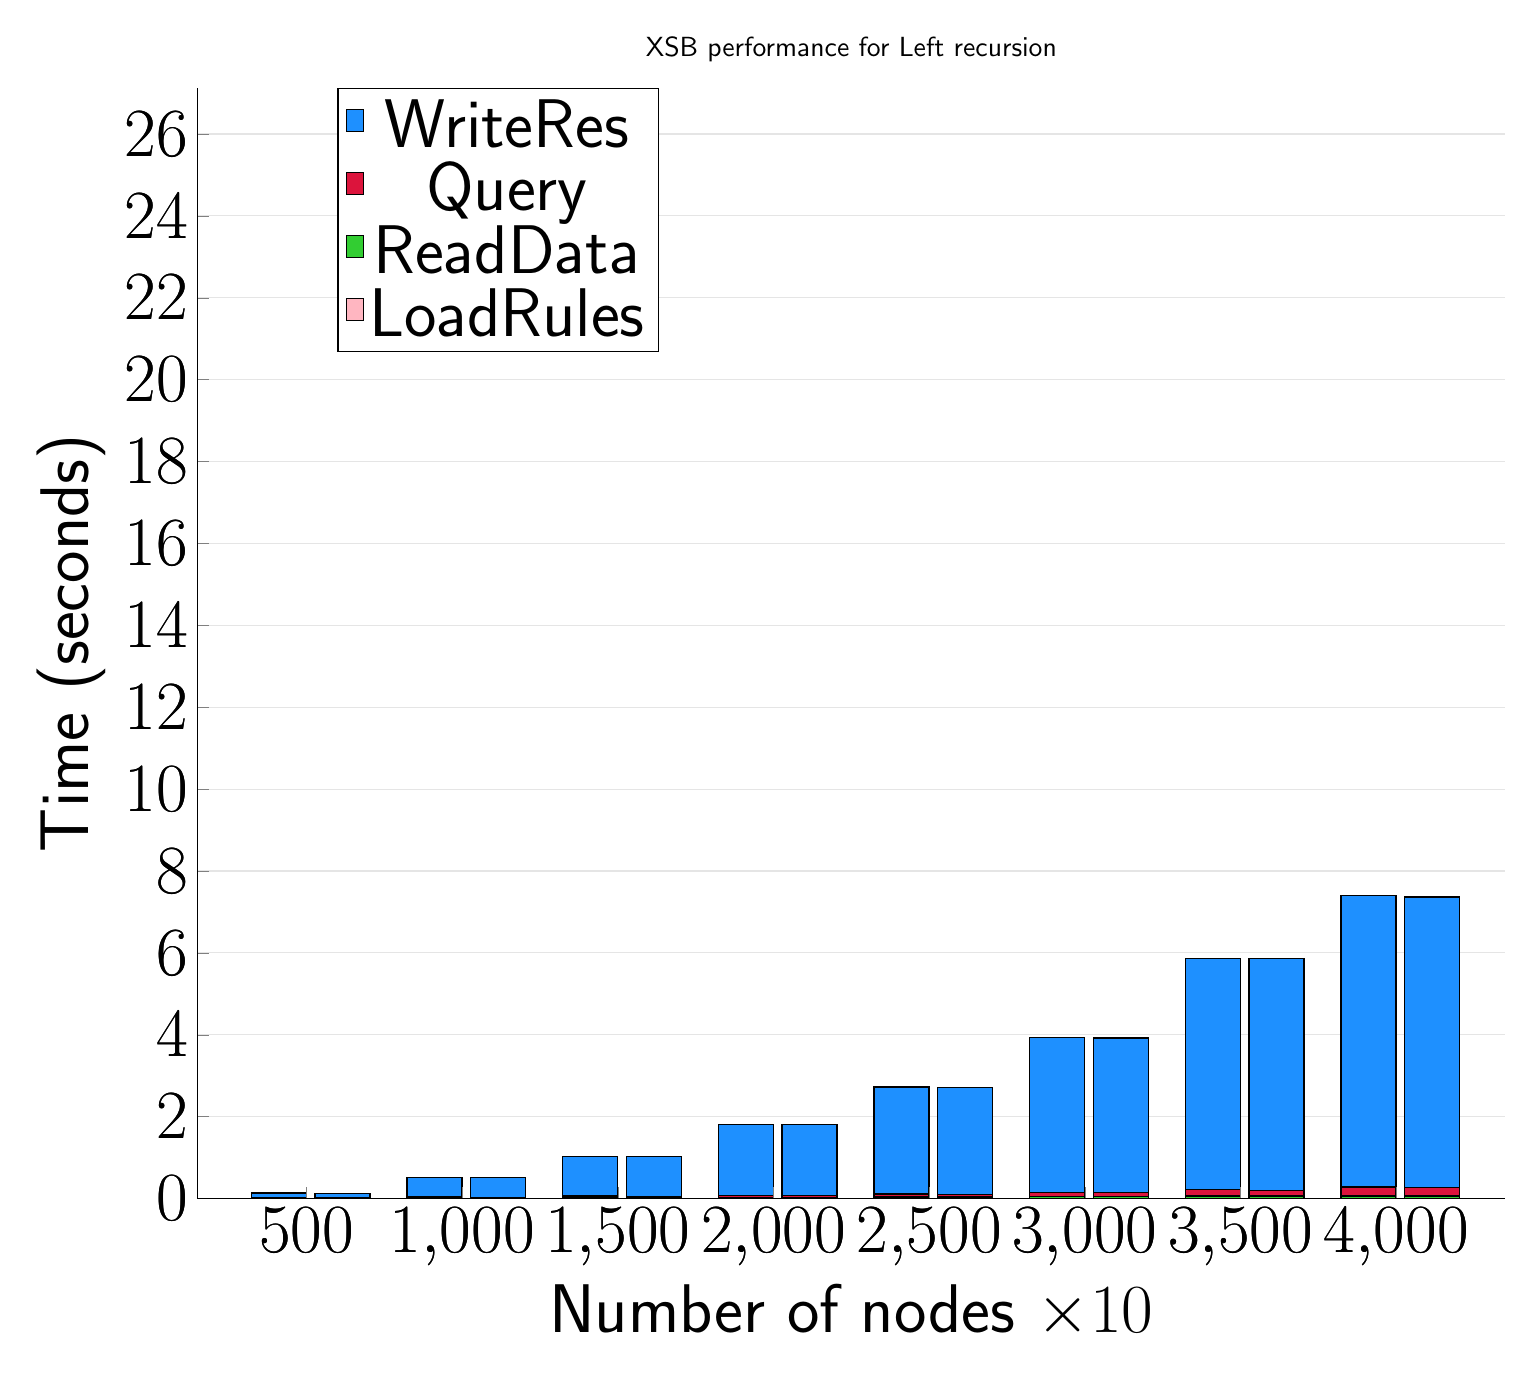
\begin{tikzpicture}
\begin{axis}[
   ybar stacked,
   title={XSB performance for Left recursion},
   bar shift=-10pt,
   width=1.5\textwidth,
   bar width=0.7cm,
   ymajorgrids, tick align=inside,
   major grid style={draw=gray!20},
   xtick=data,
   ymin=0, ymax=27.127176920572918,
   axis x line*=bottom,
   axis y line*=left,
   enlarge x limits=0.1,
   legend style={
       at={(0.23, 1)},
       anchor=north,
       legend columns=1,
       font=\Huge,
   },
   ylabel={Time (seconds)},
   xlabel={Number of nodes $\times 10$},
   label style={font=\Huge},
   tick label style={font=\Huge},
]
\addlegendimage{fill=DodgerBlue, draw=black, line width=0.2pt}
\addlegendentry{WriteRes}
\addlegendimage{fill=Crimson, draw=black, line width=0.2pt}
\addlegendentry{Query}
\addlegendimage{fill=LimeGreen, draw=black, line width=0.2pt}
\addlegendentry{ReadData}
\addlegendimage{fill=LightPink, draw=black, line width=0.2pt}
\addlegendentry{LoadRules}
\addplot +[fill=LightPink, draw=black, line width=0.5pt] coordinates {
    (500, 0.004966259002685547)
    (1000, 0.005131324132283527)
    (1500, 0.004653294881184897)
    (2000, 0.004231373469034829)
    (2500, 0.004247983296712239)
    (3000, 0.004293918609619137)
    (3500, 0.004693269729614257)
    (4000, 0.004444281260172523)
};
\addplot +[fill=LimeGreen, draw=black, line width=0.5pt] coordinates {
    (500, 0.010600646336873368)
    (1000, 0.017144997914632133)
    (1500, 0.0251193841298421)
    (2000, 0.028411626815795902)
    (2500, 0.036819060643514034)
    (3000, 0.046518405278523765)
    (3500, 0.05590542157491046)
    (4000, 0.06203301747639974)
};
\addplot +[fill=Crimson, draw=black, line width=0.5pt] coordinates {
    (500, 0.0029753843943277967)
    (1000, 0.0142357349395752)
    (1500, 0.02893892923990887)
    (2000, 0.04669904708862307)
    (2500, 0.07153693834940593)
    (3000, 0.10205626487731943)
    (3500, 0.15358495712280298)
    (4000, 0.21476236979166666)
};
\addplot +[fill=DodgerBlue, draw=black, line width=0.5pt] coordinates {
    (500, 0.11543035507202154)
    (1000, 0.47952556610107416)
    (1500, 0.9730320771535231)
    (2000, 1.73569933573405)
    (2500, 2.6152597268422437)
    (3000, 3.779862324396771)
    (3500, 5.656349817911784)
    (4000, 7.127176920572917)
};
\end{axis}
\begin{axis}[
   ybar stacked,
   bar shift=13pt,
   width=1.5\textwidth,
   bar width=0.7cm,
   ymajorgrids, tick align=inside,
   major grid style={draw=none},
   xtick=data,
   ymin=0, ymax=27.127176920572918,
   axis x line*=none,
   axis y line*=none,
   enlarge x limits=0.1,
   label style={font=\Huge},
   tick label style={font=\Huge},
]
\addplot +[fill=LightPink, draw=black, line width=0.5pt] coordinates {
    (500, 0.0043983333333333366)
    (1000, 0.0036113333333333344)
    (1500, 0.0035723333333333336)
    (2000, 0.003583)
    (2500, 0.00308)
    (3000, 0.004263333333333337)
    (3500, 0.0046926666666666636)
    (4000, 0.004095666666666667)
};
\addplot +[fill=LimeGreen, draw=black, line width=0.5pt] coordinates {
    (500, 0.00975666666666667)
    (1000, 0.014732333333333333)
    (1500, 0.024073)
    (2000, 0.028184999999999998)
    (2500, 0.033819999999999996)
    (3000, 0.04633166666666667)
    (3500, 0.055771666666666664)
    (4000, 0.061406666666666665)
};
\addplot +[fill=Crimson, draw=black, line width=0.5pt] coordinates {
    (500, 0.0029769999999999966)
    (1000, 0.014081999999999999)
    (1500, 0.028643000000000002)
    (2000, 0.04636833333333334)
    (2500, 0.069826)
    (3000, 0.10206466666666668)
    (3500, 0.14394099999999999)
    (4000, 0.21151266666666668)
};
\addplot +[fill=DodgerBlue, draw=black, line width=0.5pt] coordinates {
    (500, 0.11326433333333334)
    (1000, 0.4781503333333334)
    (1500, 0.9658199999999999)
    (2000, 1.730109)
    (2500, 2.611098666666667)
    (3000, 3.767497)
    (3500, 5.653893)
    (4000, 7.086441666666666)
};
\end{axis}
\end{tikzpicture}

\end{document}
